% Template for ICIP-2019 paper; to be used with:
%          spconf.sty  - ICASSP/ICIP LaTeX style file, and
%          IEEEbib.bst - IEEE bibliography style file.
% --------------------------------------------------------------------------
\documentclass{article}
\usepackage{spconf,amsmath,graphicx}
\usepackage{hyperref}

% Title.
% ------
\title{
  Using machine learning to predict pathological complete response and relapse-free survival outcomes to improve patient stratification and treatment}

\name{Jeffrey Adjei, Euan Deas, William Sephton, Simon Stubbs, Grace Otuagomah }
\address{Univeristy of Nottingham\\Nottingham, United Kingdom}
%
\begin{document}
%\ninept
%
\maketitle
%
\begin{abstract}
  Breast cancer remains a leading health concern globally, with pathological complete response (PCR) and relapse-free survival (RFS) serving as critical metrics for treatment efficacy. Machine learning offers a promising avenue to improve personalized cancer care by predicting these outcomes pre-chemotherapy. This study aims to develop and evaluate machine learning models that predict PCR (classification task) and RFS (regression task) using clinical and MRI-derived features from the I-SPY 2 trial dataset. The methodology includes data preprocessing, feature selection, dimensionality reduction, and model training with Support Vector Methods being chosen as the optimal models for both tasks. The classification model achieved a peak accuracy of 75\% for PCR prediction, albeit with challenges in handling class imbalance. The regression model, while robust against outliers, struggled to deliver precise RFS predictions. Despite these limitations, this research underscores the potential of machine learning in enhancing treatment stratification, paving the way for refined predictive models and broader clinical integration.
\end{abstract}
%
\begin{keywords}
  Breast Cancer, Machine Learning, Pathological Complete Response (pCR), Relapse-Free Survival (RFS)
  Support Vector Machines (SVM), Patient Stratification, Personalized Medicine, MRI-Derived Features
\end{keywords}
%
\section{Introduction}
\subsection{Background}

The application of machine learning in cancer treatment is an expansive and continuously evolving field of research. Among various types of cancer, breast cancer stands as the most prevalent form among women in the UK. Chemotherapy is a common treatment strategy used to reduce the size of locally advanced tumours before surgery. However, this approach is not always effective -  only 21\% of patients achieve a pathological complete response (PCR) after surgery,  a result associated with improved chances of cure and extended relapse-free survival (RFS). The remaining 79\% of patients experience residual disease, leading to varied prognoses\cite{spring2020pathologic}. Early prediction of PCR and RFS before chemotherapy could  enhance patient stratification and facilitate the development of more personalized treatment plans.

\subsection{Aim}

The aim of this project is to develop machine learning models that predict pathological complete response (PCR) as a classification problem and relapse-free survival (RFS) as a regression problem, utilizing pre-chemotherapy clinical and MRI-derived features. The models will be trained on data from the I-SPY 2 Trial\cite{newitt2021acr}, which includes 11 clinical features and 107 MRI-based features extracted from tumour regions. Different machine learning models and techniques will be trialled to determine the most effective approach for each prediction task. By accurately predicting PCR and RFS, this project aims to contribute to more personalized treatment strategies for breast cancer patients, aiding clinicians in better patient stratification and decision-making.

\section{Related Work}

Machine learning (ML) has shown considerable promise in guiding personalized treatment decisions in breast cancer care, particularly in predicting pathological complete response (PCR) to neoadjuvant chemotherapy. Achieving PCR at surgery is strongly associated with improved long-term outcomes, such as prolonged relapse-free survival. However, only 21\% of patients receiving chemotherapy achieve a PCR, with the remaining 79\% experiencing residual disease and varied prognoses \cite{spring2020pathologic}. Consequently, the development of accurate supervised prediction models can aid in patient stratification, sparing those unlikely to benefit from chemotherapy while optimizing treatment efficiency.

Recent studies have employed a range of ML techniques to integrate multi-modal patient data, including clinical variables (e.g., age, tumour histology, hormone receptor status), molecular biomarkers (e.g., HER2, PgR expression), and imaging-derived features, to improve PCR prediction. For example, one study \cite{Zhao2024} focused on clinicopathological features alone, evaluating various models' performance using AUC scores. While a machine learning model outperformed logistic regression in classification efficacy, the results were still relatively comparable. This research demonstrated the potential of ML models to predict PCR after neoadjuvant chemotherapy, showing both robust discrimination and calibration.

Other research has focused on improving classification efficacy in related areas, such as sentinel lymph node biopsy (SLNB) for staging axillary lymph nodes in clinically node-negative breast cancer patients. While many SLNB results are negative, and a substantial number of SLNB-positive patients do not have additional nodal metastases, accurately identifying those with extensive nodal involvement remains challenging. Predictive models in this domain vary in accuracy due to the complexity of axillary metastasis and the difficulty in capturing non-linear relationships among predictive factors. Artificial neural networks (ANNs) have been explored as a method to better model these non-linear interactions, potentially improving preoperative predictions of nodal status. By applying ANN models to commonly available clinical and pathological variables, patients could be classified into distinct risk groups (N0, N1, N2), thus guiding personalized surgical decision-making \cite{Dihge2019}. This approach could help identify patients unlikely to benefit from SLNB, reducing unnecessary interventions and improving the management of axillary disease.

Further investigations into artificial intelligence frameworks have demonstrated their applicability to various subtypes of breast cancer, including triple-negative and hormone receptor-positive disease. By enhancing predictive accuracy, these tools hold the potential to inform therapy decisions, allowing oncologists to better target neoadjuvant chemotherapy, minimize unnecessary toxicity, and streamline patient pathways toward more favorable outcomes.

\section{Method}

The machine learning pipeline for this project follows the standard sequence of data preparation, model selection, hyperparameter tuning, and model training. The process begins with data cleaning, followed by optional normalization and dimensionality reduction. After that, we explore different machine learning models and their respective hyperparameters. Model performance is initially assessed using a portion of the available data through cross-validation. The final selected model(s), along with the tuned hyperparameters, are then trained on the full dataset for final evaluation.

\subsection{Data Cleaning}

In the preprocessing phase, missing values in the dataset were imputed with the median value of each feature. For binary features such as 'pCR Outcome' (pathological complete response), missing values were replaced with the more frequent value (either 0 or 1) based on the higher frequency observed in the data. This imputation method was chosen to minimize the impact of missing data and maintain the overall distribution of the features.

\subsection{Normalisation}

Normalization was applied to the dataset to standardize the scale of the features. Each data point was rescaled so that all features, excluding the key features 'ER', 'HER2', 'Gene', and the target features 'pCR Outcome' and 'RelapseFreeSurvival' (RFS Outcome), had an L2 norm of one. This vector normalization ensures that all features are on the same scale, which is especially important for distance-based models like Support Vector Machines (SVMs), without distorting the relative importance of features.

\subsection{Feature Selection}

For the regression task (predicting RelapseFreeSurvival), Recursive Feature Elimination (RFE) was used in combination with a Random Forest Regressor. RFE iteratively removes the least important features, allowing the model to focus on the most predictive features. This ensures that the final model is both efficient and effective, utilizing only the features that contribute most to the prediction of RFS.

\subsection{Dimension Reduction}

To reduce the dimensionality of the feature set for the classification problem, Principal Component Analysis (PCA) was applied to all features except for the key features ('ER', 'HER2', 'Gene') and the target variables ('pCR Outcome' and 'RelapseFreeSurvival'). The number of principal components was chosen such that over 95\% of the variance in the data was retained. This step serves to eliminate noise and reduce the complexity of the dataset while preserving the majority of the original information.

\subsection{Model Selection and Hyperparameter Tuning}

Various machine learning models were explored for both classification and regression tasks, using k-fold cross-validation to assess the models' generalization capabilities and to find the best hyperparameters. For the classification task (predicting 'pCR Outcome'), Support Vector Classification (SVC) was chosen, while Support Vector Regression (SVR) was employed for the regression task (predicting 'RelapseFreeSurvival'). Hyperparameters for both models were optimized through the nested cross-validation mentioned previously, where a predefined parameter grid was explored using grid search. This method allows for the identification of the best hyperparameters by assessing their performance on the available data while avoiding overfitting.

\subsection{Model Training and Evaluation}

Once the hyperparameters were tuned, the final models (SVR for regression and SVC for classification) were trained on the entire dataset using the selected hyperparameters. For the final training, however, we used a standard 80:20 data split, where 80\% of the data was used for training the models, and the remaining 20\% was used for testing. This split ensured that the models were evaluated on a separate set of data, providing an unbiased measure of performance. The performance metrics were reported based on classification accuracy for the SVC model and mean absolute error (MAE) for the SVR model.

\section{Evaluation}

The dataset used to train the model is a simplified version of the publicly available dataset from The American College of Radiology Imaging Network (ACRIN) I-SPY 2 Trial \cite{newitt2021acr}. This dataset was generated to assess the effectiveness of quantitative diffusion-weighted imaging (DWI) for evaluating breast cancer response to neoadjuvant chemotherapy (NAC). The dataset comprises data from 400 patients, each with 118 features. These features are divided into two categories: 11 clinical features (e.g., patient age, tumour stage, lymph node status, etc.) and 107 MRI-based features extracted from tumour regions using a radiomics feature extraction package. While all clinical data, except for age, are categorical, the MRI-based features are continuous. The dataset also includes two target variables: a binary pathological complete response (PCR) classification and a continuous relapse-free survival (RFS) time.

Training models on this dataset presents several challenges. One key issue is the importance of retaining critical clinical features - specifically, 'ER', 'HER2', and 'Gene' - during feature selection, as they are highly relevant to the prediction of PCR and RFS. Another challenge lies in the substantial amount of missing data, particularly in the 'Gene' feature, which was absent for 88 patients. Various data imputation methods were tested to address this issue. However, the most significant challenge is the relatively small sample size of 400 patients coupled with the large number of features. This imbalance creates a high risk of overfitting, which can lead to poor generalization when applied to unseen data. Additionally, the class distribution for PCR is imbalanced, with more instances of non-PCR cases. To mitigate these issues, cross-validation was employed, although the small sample size required careful management of the number of folds to maintain balance.

For PCR classification, the Support Vector Classification (SVC) model outperformed other models during testing. Cross-validation yielded a mean accuracy of 62.25\%, with the best fold achieving 79\% accuracy and the worst fold at 23\%. The optimal model parameters were a balanced class weight, Radial Basis Function (RBF) kernel, C = 1, and gamma = 0.01. Retraining the model on an 80:20 train-test split with these parameters resulted in an accuracy of 75\%. The model performed better at predicting non-PCR cases, with an F1 score of 83\%, compared to 50\% for predicting PCR-positive cases. This imbalance is reflected in the confusion matrix shown in Figure \ref{fig:f1}, which highlights the model's tendency to predict non-PCR outcomes more accurately. The ROC curve (Figure \ref{fig:f2}) suggests that the model has moderate discriminatory power, performing slightly better than random guessing but not excelling in class separation.

\begin{figure}
  \centering
  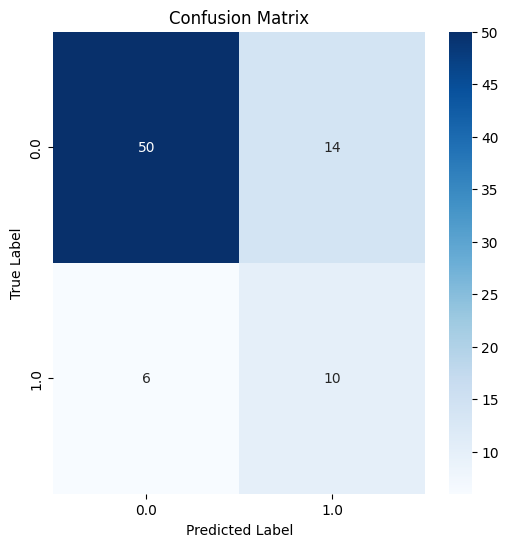
\includegraphics[width=0.75\linewidth]{cm.png}
  \caption{SVC Confusion Matrix}
  \label{fig:f1}
\end{figure}

\begin{figure}
  \centering
  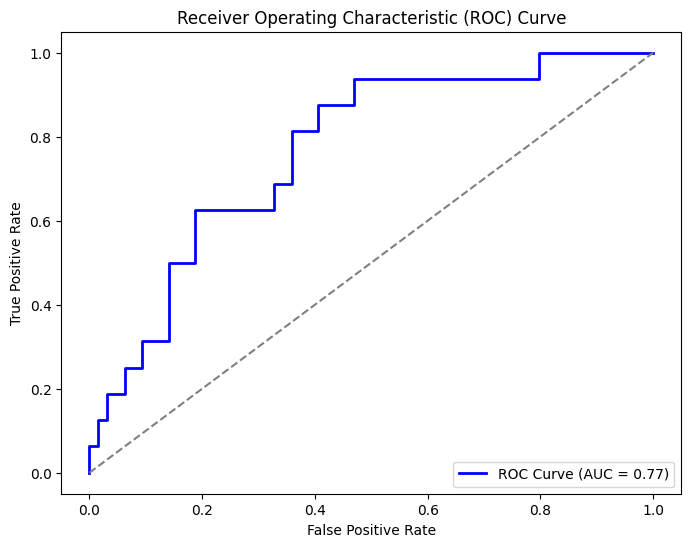
\includegraphics[width=0.75\linewidth]{roc.png}
  \caption{SVC Confusion Matrix}
  \label{fig:f2}
\end{figure}

For RFS regression, the Support Vector Regressor (SVR) was selected after testing various models. Cross-validation revealed a mean squared error (MSE) of 739.18, an R-squared value of -0.0074, and a mean absolute error (MAE) of 21.2267, indicating suboptimal performance. The best parameters identified through cross-validation were an RBF kernel, C = 1, and epsilon = 0.2. However, training the model on an 80:20 split of the dataset resulted in an MSE of 797.89, an R-squared value of 0.0002, and an MAE of 21.64. These results indicate that the model struggles to make accurate predictions and shows little improvement over predicting the mean of the target variable for all instances. The lack of precision and poor model fit suggest that further improvements in feature selection, data preprocessing, or model architecture may be necessary for better regression performance.

\section{Discussion}

Both the Support Vector Classification (SVC) and Support Vector Regression (SVR) models present distinct advantages and challenges, making them well-suited to different aspects of this project. Understanding these characteristics is crucial for interpreting the results and justifying their selection.

The SVC model is highly effective for high-dimensional datasets, like the one used in this study, due to its ability to generate complex decision boundaries. This is particularly important in situations where there are many features, as it helps the model distinguish between classes based on subtle patterns in the data. Moreover, the SVC model benefits from margin maximization, which enhances its ability to generalize to unseen data. This is a significant advantage in practical applications where robustness to new, unseen cases is essential.

However, SVC models do have some limitations. One major challenge is the need for careful selection and tuning of hyperparameters. The choice of kernel, for example, is critical—an incorrect kernel can drastically degrade model performance. Additionally, SVC models can be computationally expensive, particularly when applied to large datasets. For smaller or less complex datasets, other machine learning methods might be more efficient in terms of processing time.

Despite these drawbacks, the advantages of the SVC model outweigh the disadvantages in this case. Time and effort have been invested in tuning the hyperparameters, and the availability of a well-curated dataset has streamlined the feature selection process, allowing for more accurate model training. Therefore, the SVC model remains a strong choice for this classification task.

The SVR model offers a key advantage with its robustness to outliers. By using a margin of tolerance, SVR focuses on modelling the general trend of the data rather than fitting to every individual data point. This is particularly beneficial for regression tasks where noise or extreme outliers might otherwise have a disproportionate effect on model performance. Similar to SVC, SVR is well-suited to high-dimensional data, which increases its versatility and applicability to a wide range of problems.

However, SVR shares some of the same challenges as SVC, notably its computational complexity. As with SVC, SVR can be slow to process large datasets, and the time required for training and testing may be a concern when efficiency is a priority. Furthermore, the model requires careful hyperparameter tuning to achieve optimal performance. While we have dedicated time to fine-tune the SVR model, the reliance on hyperparameter optimization remains a challenge, particularly in situations with limited resources or time constraints.

In summary, while SVR shares several advantages with SVC, such as handling high-dimensional data and mitigating the effects of outliers, it also faces similar drawbacks. Nevertheless, careful tuning of the hyperparameters and the relatively small dataset used in this study make SVR an appropriate choice for predicting relapse-free survival (RFS), although as seen in the evaluation it struggled as expected with the data set.

\section{Conclusion}

Our results demonstrate the feasibility of employing machine learning techniques to predict pathological complete response (PCR) and relapse-free survival (RFS) in breast cancer patients. The support vector classification (SVC) model performed well in identifying cases where PCR was not achievable, underscoring its ability to discern key patterns in high-dimensional datasets. However, it faced challenges in accurately predicting cases where PCR was achieved, likely due to the imbalance in the dataset. Similarly, while the support vector regression (SVR) model provided a foundation for predicting RFS, its overall performance was suboptimal, suggesting that further refinement in model selection, feature engineering, or data preprocessing may be required. These findings highlight the promise of machine learning in personalizing breast cancer treatment, while also emphasizing areas for improvement.

Future work should prioritize addressing dataset limitations, particularly by incorporating a larger and more balanced dataset to enhance model performance. Balanced datasets could not only improve the classification model's ability to predict PCR-positive cases but also improve the regression model's predictive accuracy for RFS. Exploring advanced machine learning approaches, such as ensemble methods or neural networks, may also prove beneficial for capturing complex relationships within the data. Ultimately, these efforts would contribute to developing robust, clinically applicable models that can improve patient stratification and inform more effective, individualized treatment strategies.

\bibliographystyle{unsrt}
\bibliography{refs}

\begin{table}[bp]
  \begin{tabular}{|p{2cm}|p{2.5cm}|p{2.5cm}|p{2.5cm}|p{2.5cm}|p{2.5cm}|}
  \hline
  \textbf{Task and Weighting} & \textbf{Data Preprocessing (10\%)} & \textbf{Feature Selection (25\%)} & \textbf{ML Method Development (25\%)} & \textbf{Method Evaluation (10\%)} & \textbf{Report Writing (30\%)} \\ \hline
  Ejiroghene Otuagomah & 20\% & 20\% & 16\% & 16\% & 20\% \\ \hline
  Jeffrey Adjei & 20\% & 20\% & 16\% & 16\% & 20\% \\ \hline
  Simon Stubbs & 20\% & 20\% & 16\% & 16\% & 20\% \\ \hline
  Euan Deas & 20\% & 20\% & 36\% & 36\% & 20\% \\ \hline
  William Sephton & 20\% & 20\% & 16\% & 16\% & 20\% \\ \hline
  \end{tabular}
  \end{table}

\end{document}
